\documentclass[11pt]{article}

\usepackage[margin=1in]{geometry}
\usepackage{amsmath,amssymb}
\usepackage{tikz}

\usepackage[colorlinks=true,
            linkcolor=blue,
            urlcolor=blue,
            citecolor=blue]{hyperref}

\title{Calculus Refresher}
\author{Deepak Venkatesh}
\date{\today}

\begin{document}

\maketitle
\tableofcontents
\newpage

\section{Personal Notes}

These notes are a concise collection of derived problems from the examples from Calculus books mentioned in the references.

\newpage

\section{Calculus I}

\subsection{Reading Limits from a Graph}

From the graph of $y=h(x)$ below, find $\lim_{x\to a} h(x)$, if it exists, for
$$
a=1,2,3,4,5.
$$

Also state $h(a)$ whenever it is defined.

\begin{center}
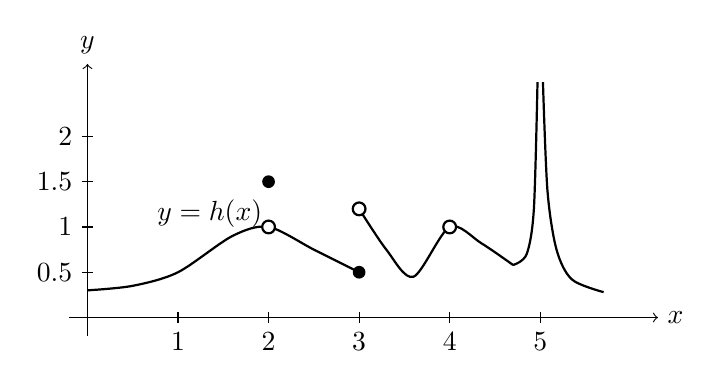
\begin{tikzpicture}[scale=1.15]

% Axes
\draw[->] (-0.2,0) -- (6.3,0) node[right] {$x$};
\draw[->] (0,-0.2) -- (0,2.8) node[above] {$y$};

% x-axis ticks
\foreach \x in {1,2,3,4,5}
  \draw (\x,0.06) -- (\x,-0.06) node[below] {$\x$};

% y-axis ticks
\foreach \y/\label in {0.5/{0.5},1/{1},1.5/{1.5},2/{2}}
  \draw (0.06,\y) -- (-0.06,\y) node[left] {$\label$};

% First curve
\draw[thick]
  plot[smooth] coordinates {
    (0,0.3)
    (0.5,0.35)
    (1,0.5)
    (1.6,0.9)
    (2,1.0)
    (2.5,0.75)
    (3,0.5)
  };

% Hole at x=2 and actual value at x=2
\draw[thick, fill=white] (2,1.0) circle (2pt);
\fill (2,1.5) circle (2pt);

% Closed point at x=3 from the left piece
\fill (3,0.5) circle (2pt);

% Second curve starting with a jump at x=3
\draw[thick]
  plot[smooth] coordinates {
    (3,1.2)
    (3.3,0.75)
    (3.6,0.45)
    (4,1.0)
    (4.35,0.82)
    (4.7,0.58)
  };

% Open circles
\draw[thick, fill=white] (3,1.2) circle (2pt);
\draw[thick, fill=white] (4,1.0) circle (2pt);

% Curve with vertical blow-up near x=5
\draw[thick]
  plot[smooth] coordinates {
    (4.7,0.58)
    (4.85,0.7)
    (4.93,1.2)
    (4.97,2.6)
  };

\draw[thick]
  plot[smooth] coordinates {
    (5.03,2.6)
    (5.08,1.4)
    (5.18,0.75)
    (5.35,0.42)
    (5.7,0.28)
  };

% Label
\node at (1.35,1.15) {$y=h(x)$};

\end{tikzpicture}
\end{center}

\subsection*{Answer}

From the graph we read:

$$
\lim_{x\to 1} h(x)=0.5
$$

since the graph is continuous there.

$$
\lim_{x\to 2} h(x)=1
$$

even though

$$
h(2)=1.5.
$$

At $x=3$, the left-hand limit is $0.5$ while the right-hand limit is $1.2$, so

$$
\lim_{x\to 3} h(x)
$$

does not exist.

At $x=4$, the graph approaches $1$ from both sides, so

$$
\lim_{x\to 4} h(x)=1,
$$

but $h(4)$ is not defined.

As $x$ approaches $5$, the function grows without bound, so

$$
\lim_{x\to 5} h(x)
$$

does not exist as a finite number.

\subsection{Find $\displaystyle \lim_{x\to 0} \frac{\left|x\right|}{x}$}

\subsection*{Answer}

This is better visually but we can see that for $x > 0$ the functions is 1 and for $x < 0$ the function is 
-1, and at $x = 0$ the denominator is 0 and the function is undefined at that point. Therefore the limit does 
not exist at 0.

\begin{center}
\begin{tikzpicture}[scale=1.2]

% Axes
\draw[->] (-3.5,0) -- (3.5,0) node[right] {$x$};
\draw[->] (0,-1.8) -- (0,1.8) node[above] {$y$};

% x-axis ticks
\foreach \x in {-3,-2,-1,1,2,3}
  \draw (\x,0.08) -- (\x,-0.08) node[below] {$\x$};

% y-axis ticks
\foreach \y in {-1,1}
  \draw (0.08,\y) -- (-0.08,\y) node[left] {$\y$};

% Left branch: y = -1 for x<0
\draw[thick] (-3.2,-1) -- (0,-1);

% Right branch: y = 1 for x>0
\draw[thick] (0,1) -- (3.2,1);

% Open circles at x=0
\draw[thick, fill=white] (0,1) circle (2pt);
\draw[thick, fill=white] (0,-1) circle (2pt);

% Label
\node at (2.2,1.5) {$y=\dfrac{|x|}{x}$};

\end{tikzpicture}
\end{center}

\subsection{Find $\displaystyle \lim_{x\to \infty} \dfrac{1}{x}$}

\subsection*{Answer}

This will be simply 0, since denominator tends to 0 and the resultant fraction will tend to $\infty$.


\subsection{Find $\displaystyle \lim_{x\to \infty} \dfrac{7x - 2}{11x + 9}$}

\subsection*{Answer}

\[
\lim_{x\to \infty} \dfrac{7x - 2}{11x + 9} = \lim_{x\to \infty} \dfrac{7 - 2/x}{11 + 9/x} = \dfrac{7}{11}
\]

\subsection{Find $\displaystyle \lim_{x\to -\infty} \dfrac{4x^2 - 5x + 3}{x^2 + 2}$}

\subsection*{Answer}

\[
\lim_{x\to -\infty} \dfrac{4x^2 - 5x + 3}{x^2 + 2} = \lim_{x\to -\infty} \dfrac{4 - 5/x + 3/x^2}{1 + 2/x^2} = 4
\]






































































































%\section{Calculus II}

%\section{Calculus III}

\newpage
\section{References}

Marsden, Jerrold E. and Alan Weinstein,
\textit{Calculus I, II, III}.

\url{https://www.cds.caltech.edu/~marsden/volume/Calculus/}

\end{document}